\documentclass{article} % For LaTeX2e
\usepackage[preprint]{colm2025_conference}

\usepackage{microtype}
\usepackage{hyperref}
\usepackage{url}
\usepackage{booktabs}
\usepackage{graphicx}

\usepackage{lineno}

\definecolor{darkblue}{rgb}{0, 0, 0.5}
\hypersetup{colorlinks=true, citecolor=darkblue, linkcolor=darkblue, urlcolor=darkblue}

\usepackage[most]{tcolorbox}
\tcbuselibrary{listings,breakable}
\usepackage{xcolor}

\definecolor{PromptFrame}{HTML}{4B6584}   % 边框色
\definecolor{PromptBack}{HTML}{F7F9FC}    % 背景色
\definecolor{PromptTitle}{HTML}{1B1F3B}   % 标题文字色

% 适合一小段文本的盒子(不用 verbatim)
\newtcolorbox{promptbox}[2][]{%
  enhanced,
  breakable,
  colback=PromptBack,
  colframe=PromptFrame,
  boxrule=0.4pt,
  arc=1.5mm,
  outer arc=1.5mm,
  fonttitle=\bfseries,
  coltitle=PromptTitle,
  title={#2},
  left=3mm, right=3mm, top=1.5mm, bottom=1.5mm,
  attach boxed title to top left={xshift=2mm,yshift*=-2mm},
  boxed title style={colback=white,arc=1mm,outer arc=1mm},
  #1
}

% 适合直接粘贴完整 prompt(代码风、等宽字体)
\newtcblisting{promptlisting}[2][]{%
  enhanced,
  breakable,
  colback=PromptBack,
  colframe=PromptFrame,
  boxrule=0.4pt,
  arc=1.5mm,
  outer arc=1.5mm,
  fonttitle=\bfseries,
  coltitle=PromptTitle,
  title={#2},
  listing only,
  listing options={
    basicstyle=\ttfamily\small,
    breaklines=true,
    columns=fullflexible,
    keepspaces=true
  },
  left=3mm, right=3mm, top=1.5mm, bottom=1.5mm,
  attach boxed title to top left={xshift=2mm,yshift*=-2mm},
  boxed title style={colback=white,arc=1mm,outer arc=1mm},
  #1
}

\title{Pessimistic Verification for Open Ended Math Questions}

% Authors must not appear in the submitted version. They should be hidden
% as long as the \colmfinalcopy macro remains commented out below.
% Non-anonymous submissions will be rejected without review.

\author{Antiquus S.~Hippocampus, Natalia Cerebro \& Amelie P. Amygdale \thanks{ Use footnote for providing further information
about author (webpage, alternative address)---\emph{not} for acknowledging
funding agencies.  Funding acknowledgements go at the end of the paper.} \\
Department of Computer Science\\
Cranberry-Lemon University\\
Pittsburgh, PA 15213, USA \\
\texttt{\{hippo,brain,jen\}@cs.cranberry-lemon.edu} \\
\And
Ji Q. Ren \& Yevgeny LeNet \\
Department of Computational Neuroscience \\
University of the Witwatersrand \\
Joburg, South Africa \\
\texttt{\{robot,net\}@wits.ac.za} \\
\AND
Coauthor \\
Affiliation \\
Address \\
\texttt{email}
}

% The \author macro works with any number of authors. There are two commands
% used to separate the names and addresses of multiple authors: \And and \AND.
%
% Using \And between authors leaves it to \LaTeX{} to determine where to break
% the lines. Using \AND forces a linebreak at that point. So, if \LaTeX{}
% puts 3 of 4 authors names on the first line, and the last on the second
% line, try using \AND instead of \And before the third author name.

\newcommand{\fix}{\marginpar{FIX}}
\newcommand{\new}{\marginpar{NEW}}

\begin{document}

\ifcolmsubmission
\linenumbers
\fi

\maketitle

\begin{abstract}
  The key limitation of the verification performance lies in the ability of error detection. With this intuition we designed several variants of pessimistic verification, which are simple workflows that could significantly improve the verification of open-ended math questions. In pessimistic verification we conducts multiple reviews on a single proof with a special focus on certain parts, and reports false if any one of them finds an error. This simple technique significantly improves the performance across many math verification benchmarks without introducing too much extra budget. Its token efficiency even surpassed extended long-cot in test-time scaling. Self verification and correction are one of the central perspectives of reasoning and intelligence. This enables an agent to constantly refine its own reasoning or actions, and they are also critical for effectively performing long tasks such as mathematical research. We believe pessimistic verification would be especially useful for many related researches.
\end{abstract}

\section{Introduction}

Since the release of OpenAI o1~\citep{openai_openai_2024} and DeepSeek-R1~\citep{deepseek-ai_deepseek-r1_2025}, reasoning has become one of the most important topics in large language model (LLM) research within both academia and industry. Nevertheless, the scalability of the training recipe behind current large reasoning models (LRMs) is still limited by the requirement of verifiable reward. Even in math, one of the most successful domain of LRM, the absence of a generic verifiable reward still introduces significant challenges to more advanced, open-ended and long-form reasoning tasks~\citep{xu_direct_2025}.

One possible solution to this problem is through formal theorem provers such as Lean~\citep{chen_seed-prover_2025, varambally_hilbert_2025}, which could provide completely reliable verification on math proofs. However, this approach would introduce notable external budget to the AI system and their performance still largely falls behind that of provers in natural language~\citep{dekoninck_open_2025}. Another line of work focuses on leveraging the internal capability of the LLM to achieve self evolution~\citep{zuo_ttrl_2025, yu_rlpr_2025, xu_direct_2025}.

We contend that the importance of self-verification capabilities can be reflected in several key dimensions:

\begin{itemize}
  \item Effective self-verification can substantially enhance the reliability of model outputs and significantly improve overall performance. The performance IMO level math problems can be notably enhanced via a verifier-guided workflow according to \citet{huang_gemini_2025, luong_towards_2025}.
  \item Existing research indicates that the reliability of single-step task execution strongly influences the duration over which a system can operate dependably, thus introspective abilities may be particularly critical for long-horizon tasks~\citep{kwa_measuring_2025}.
  \item We further argue that a general intelligent system should possess intrinsic mechanisms for self-validation, rather than relying exclusively on external ground-truth signals or verification modules.
\end{itemize}

Intuitively we believe that the key limitation of verification lies in the ability of finding errors in a proof, which is also supported by some recent researches~\citep{pandit_hard2verify_2025}. So in this work we introduce three simple workflows which we call \textbf{simple pessimistic verification}, \textbf{vertical pessimistic verification}, and \textbf{progressive pessimistic verification}. These methods imitate the common practice of the review process of math papers, where a paper would be rejected if any one reviewer finds an error in it. They will review a given solution multiple times from different perspectives, and the whole proof will be considered false if any one review finds an error. We have conducted a series of experiments on three datasets, \textit{Hard2Verify}~\citep{pandit_hard2verify_2025}, \textit{IMO-GradingBench}~\citep{luong_towards_2025}, and our homemade \textit{QiuZhen-Bench}. The former two benchmarks are both contest-level math grading benchmarks with expert annotations. \textit{QiuZhenBench} was collected and curated from S.-T. Yau College Student Mathematics Contest and the doctoral qualifying exams fron QiuZhen college, Tsinghua University. These exams covers a wide range of topics in undergraduate-level mathematics and are well-known for their high difficulty. On all benchmarks our methods consistently show impressive improvements in error detection rate and overall f1 score, indicating their effectiveness on proof verifications.

\section{Method}

\begin{figure}[htbp]
  \centering
  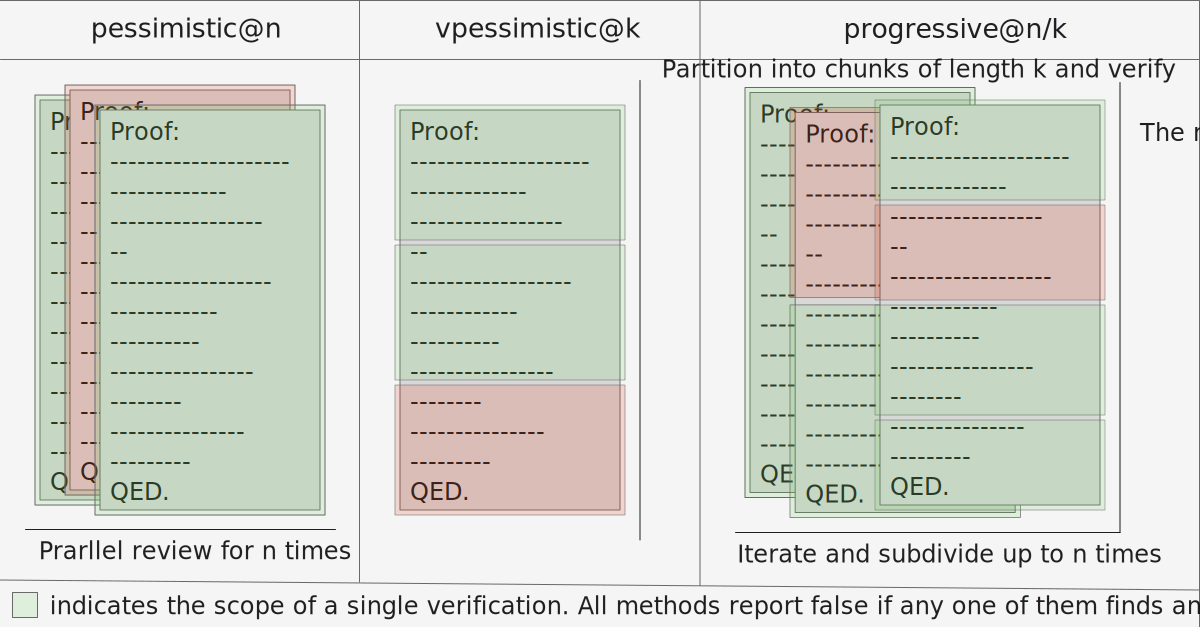
\includegraphics[width=1.0\textwidth]{pessimistic_verifiers.pdf}
  \caption{Three variants of pessimistic verification methods in this work. In following experiments they will separately be denoted as ``pes@n'', ``vp@l'', and ``prog@n/l''}
  \label{fig:pverify-methods}
\end{figure}

\subsection{Metrics}

In this work, we treat mathematical proof verification as a binary classification problem and focus on the following performance metrics:

\begin{itemize}
  \item \textbf{True Negative Rate (TNR)}: The proportion of detected errors among all erroneous proofs. This is the primary metric for evaluating the model’s ability to identify incorrect proofs.
  \item \textbf{True Positive Rate (TPR)}: The proportion of proofs classified as correct among all truly correct proofs. This helps assess the model’s proof-verification capability.
  \item \textbf{Balanced F1 Score}: The harmonic mean of TPR and TNR, providing a balanced indicator of performance when both false positives and false negatives matter. This is also the primary indicator used in \citet{pandit_hard2verify_2025}.
\begin{equation}
  \mathrm{Balanced\ F1} = \frac{2 \cdot \mathrm{TPR} \cdot \mathrm{TNR}}{\mathrm{TPR} + \mathrm{TNR}}
  \label{eq:balanced-f1}
\end{equation}
\end{itemize}

\subsection{Simple pessimistic verification}

A common strategy of enhancing model capability is through majority voting. In majority voting we run the same requests in parallel for multiple times, and choose the majority as final answer. However, this mechanism does not work on verification tasks according to our experiments and some related researches~\citep{pandit_hard2verify_2025}.

In simple pessimistic verification, we conduct multiple reviews on a single proof as majority voting, but instead of using the majority as final answer, we will constantly choose the worst verification from these reviews. As shown in Figure~\ref{fig:pes-vs-maj}, this method drasticly improves the overall performance of evaluation where majority has almost no effect.

We can roughly understand this phenomenon as follows: since the most difficult part of mathematical proof verification is detecting errors, it is likely that only a small number of evaluations can identify the critical mistakes. In this case, majority voting may actually restrict the model’s ability to uncover potential errors, while pessimistic verification further reinforces this ability.

\begin{figure}[htbp]
  \centering
  \includegraphics[width=1.0\textwidth]{./pes_vs_maj.pdf}
  \caption{The comparion of simple pessimistic verification and majority voting. The former exhibits steady performance gains as sampling budget increases, whereas the latter shows almost no changes in performance.}
  \label{fig:pes-vs-maj}
\end{figure}

\subsection{Vertical pessimistic verification}

In spite of simply applying multiple reviews on the whole proof, we also explored a pessimistic verification from another dimension. As shown in Figure~\ref{fig:vertical-prompting}, we adopted a special prompting method and require the LLM to focus on a certain part of the proof, and try looking deep into these contents to find errors. Vertical pessimistic verification adopts a hyperparameter $l$, it first splits the whole proof into chunks with $l$ lines, and create a series of parallel review tasks for each chunk. Although this method only goes through the proof once, we also witnessed improved performance in error detection and even a higher scaling efficiency compared to simple pessimistic verification. 

\begin{figure}[htbp]
  \centering
  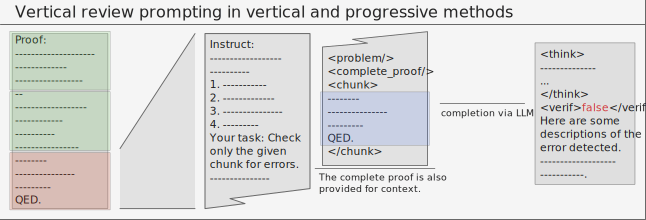
\includegraphics[width=1.0\textwidth]{./vertical_review_prompting.pdf}
  \caption{The vertical review prompting method used in vertical pessimistic verification and progressive pessimistic verification.}
  \label{fig:vertical-prompting}
\end{figure}

\subsection{Progressive pessimistic verification}

Combining the mechanism of both simple and vertical methods we can create a progressive pessimistic verification method. This method starts from the whole proof verification, and then progressively subdivide the proof for up to $n$ times. Each chunk is restricted to contain at least $l$ lines. After this process we can create at most $2^n - 1$ different verification requests on a single proof at different scales. This approach eventually achieved the highest performance under certain sampling budget.

\subsection{Pruning in pessimistic verification}

The mechanism of pessimistic verification also enables pruning in the process. We can implement serial execution at certain levels and stop subsequent checks once an earlier validation detects an error. This allows us to effectively reduce computational resource consumption without sacrificing performance. However, running in a serial manner also slows down execution speed, so we need to find a balance between speed and cost.

The progressive verification approach naturally supports pruning. It can run each round of verification in order from coarse to fine, filtering out incorrect answers step by step. Therefore, in our experiments, pruning is enabled by default for this method, and other approaches can be applied in a similar way. Pruning is especially useful when most of the examples in the dataset are negative examples.

\section{Experiments}

\subsection{Datasets and settings}

In our experiments we primarily use three datasets for evaluation, and we constantly use the same prompt and workflow setting across all these dataset. Here are some descriptions about them:

\begin{itemize}
  \item \textbf{IMO-GradingBench}~\citep{luong_towards_2025}. This dataset contains 1,000 human-graded solutions to IMO-level proof problems from IMO-ProofBench~\citep{luong_towards_2025}, from which we selected a subset with 300 samples for evaluation. This is a challenging test of fine-grained mathematical proof evaluation.
  \item \textbf{Hard2Verify}~\citep{pandit_hard2verify_2025}. Hard2Verify contains 200 challenging problems and solutions from recent math conpetitions such as IMO and Putnam. The solutions are generated by strong models such as GPT-5 and Gemini 2.5 Pro and annotated by humans.
  \item \textbf{QiuZhen-Bench}. This is a homemade collection of advanced math problems, with questions sourced from challenging university-level math competitions. It serves as a supplement to the previous two elementary math competition problem datasets. We randomly selected a subset of 300 problems, had them answered by GPT-5-mini, and used GPT-5 for labeling. This subset can be used to evaluate the performance of weaker models. You can refer to Appendix~\ref{sec:qiuzhen-bench} for more details.
\end{itemize}

All evaluation in our experiments was conducted at the response level, and for IMO-GradingBench, only the responses that obtained fully 7 points are considered correct, otherwise they will all be considered false. And aside from our experiments, we will simply use single pass verification with different reasoning effort setting as the baseline, since we already know that majority voting has almost no effect on evaluation. In all our experiments we set the temperature parameter to 1.0 to ensure the diversity of the response.

\subsection{Performance}

\begin{figure}[htbp]
  \centering
  \includegraphics[width=1.0\textwidth]{tnr_f1_comparison.pdf}
  \caption{The main results on IMO-GradingBench. Thinking mode is enabled for all models if possible, and the reasoning effort of gpt series model is set to medium. This method constantly improves the classification performance across all tested models.}
  \label{fig:main-results}
\end{figure}

\subsection{Scaling potential of pessimistic verification}

\subsection{Case study}

\section{Related work}

Using LLM for evaluation or verification tasks is a natural idea. At the early development stage of LLM, some works have already tried this method on traditional tasks in natural language processing, such as text summarization~\citep{liu_g-eval_2023}, dialog generation~\citep{liu_g-eval_2023}, and machine translation~\citep{zheng_judging_2023}. This approach has achieved some results, but several problems still remain, such as scoring bias~\citep{li_evaluating_2025} and self-inconsistency~\citep{haldar_rating_2025}.

The open-ended math problem lies between the math answering problem and other evaluation problems. It lacks simple and direct means of verification, but its correctness is entirely objective. Existing works in this area primarily focus on the alignment of LLM grading and that of humans. Some of them proposed certain agentic workflows that could enhance this ability~\citep{mahdavi_refgrader_2025, mahdavi_scaling_2025}. Reinforcement learning on manually annotated data also exhibited effectiveness on the evaluation of mathematical proofs~\citep{dekoninck_open_2025}. However, these methods lack the scalability in further enhancing the performance, and they cannot distinguish performance improvements brought by subjective preference alignment from those resulting from objectively discovering new errors. Some work also highlights the importance of error detection, as this is the key ability that separates strong verifiers from weaker ones~\citep{pandit_hard2verify_2025}. Before the release of this work, there is no well-known method that could leverage test-time scaling to obtain better evaluation performance other than scaling long chain of thought~\citep{pandit_hard2verify_2025}.

\section{Conclusion and discussion}

In this work we proposed several variants of pessimistic verification method, which exhibits strong performance and even higher scaling potential than long chain of thought on the evaluation of open-ended math problems. These methods construct multiple different verification queries for a single mathematical proof in different ways, and deems the proof incorrect if any one of these queries determines it to be wrong.

Beyond the existing concrete implementations and results, we believe that the error-centered idea behind pessimistic verification is what truly deserves attention. This approach will naturally make the verification of mathematical problems increasingly stringent, which may also align with the field’s gradual trend toward greater formalization and rigor. It may likewise help guide large language models away from merely computing correct answers and toward generating fully rigorous proofs.

We can also envision several direct applications of pessimistic verification:

\begin{itemize}
  \item Using pessimistic verification in math or code related workflows can further improve the reliability of the response, especially for long-form tasks.
  \item This method can further push the capability frontier of state-of-the-art large models, so there is an opportunity to incorporate it into the training pipeline to further raise the upper limit of large models’ abilities in executing verification and rigorous proof tasks.
\end{itemize}

We are also excited about the future works inspired by our pessimistic verification.

\bibliography{pverify}
\bibliographystyle{colm2025_conference}

\appendix
\section{Appendix}

\subsection{Detail in QiuZhen-Bench}\label{sec:qiuzhen-bench}

QiuZhen-Bench is a dataset covering a wide range of topics in advanced math, including analysis, algebra, machine learning theory, geometry, topology, probability, statistics and theoretical physics. We have collected 143 exam papers from S.-T. Yau College Student Mathematics Contest since 2010, and the doctoral qualifying exams fron QiuZhen college, Tsinghua University since 2023, and required GPT-5 to extract and reformat problems directly from the PDF files. Manual spot checks did not reveal any errors in these extracted contents, indicating the strong capability of GPT-5 in doing this task. We firstly divide the exam papers into pages, and for each page we used the following prompt for extraction:

\begin{promptlisting}{system prompt}
You are a meticulous exam parsing assistant.
Extract ALL distinct problems from the provided text chunks.
Return ONLY valid JSON (no commentary). Focus on problem statements; exclude answers and solutions.
\end{promptlisting}

\begin{promptlisting}{user prompt}
Task: Parse the following exam/contest page images to extract problem statements.
Requirements:
- Identify each separate problem with its number or index if present.
- Preserve math using Markdown and LaTeX (inline `$...$`, display `$$...$$`).
- Do not infer content; only use what appears in the images.
- Only include problems written in English; skip non-English (e.g., Chinese).
- If a problem is mixed-language, include only the English statement; otherwise skip.
- If a problem spans multiple pages in this chunk, include the full statement.
Output strictly as JSON array of objects with keys:
  - problem_number: string (e.g., '1', 'II-3', 'A.1'; use 'unknown' if missing)
  - markdown_statement: string (problem text in Markdown; no solution)
  - section: string|null (e.g., 'Analysis', 'Geometry', or null)
  - tags: array of strings (optional keywords, may be empty)
  - source_pages: array of integers (page numbers within this PDF chunk)
Return ONLY JSON.

fSource: {source.rel_path}\nPages: {chunk.start_page}-{chunk.end_page}
\end{promptlisting}

The problems that spans across two pages is extracted by part and combined in the following processing logic. This results in a dataset containing 1,054 problems in total. Here we provide some samples from this dataset:

\begin{promptbox}{Yau contest 2015, applied math}
Let $G$ be graph of a social network, where for each pair of members there is either no connection, or a positive or a negative one.  An unbalanced cycle in $G$ is a cycle which have odd number of negative edges. Traversing along such a cycle with social rules such as friend of enemy are enemy would result in having a negative relation of one with himself!  A resigning in $G$ at a vertex $v$ of $G$ is to switch the type (positive or negative) of all edges incident to $v$.  Question: Show that one can switch all edge of $G$ into positive edges using a sequence resigning if and only if there is no unbalanced cycle in $G$.
\end{promptbox}

\begin{promptbox}{QiuZhen qualifying 2024 spring, theoretical physics}
$\Pi_{\mu\nu}(q)$ via dimensional regularization (35 points)

At one-loop, the photon propagator in QED receives the correction

$$i\,\Pi_{\mu\nu}(q) = - \int \frac{d^4 p}{(2\pi)^4} \, \mathrm{Tr} \left( i\,\gamma^\nu \, \frac{i}{\not p + \not q - m} \, i\,\gamma^\mu \, \frac{i}{\not p - m} \right),$$

where $\gamma_\mu$ is the gamma matrix and $\not p = p^\mu \gamma_\mu$.

i) 10' Show that this expression can be written as

$$i\,\Pi_{\mu\nu}(q) = -i \int \frac{d^4 p}{(2\pi)^4} \, \frac{N_{\mu\nu}}{D},$$

where

$$N_{\mu\nu} = \operatorname{tr}\,[\gamma_\nu(\not p + \not q + m)\gamma_\mu(\not p - m)]\,, \qquad \frac{1}{D} = \int_0^1 d\alpha \, \frac{1}{D},$$

with

$$D = \big[\,l^2 + \alpha(1-\alpha) q^2 - m^2 + i\epsilon\,\big]^2, \qquad \text{where } l = p + \alpha q.$$

ii) 10' Evaluate $N_{\mu\nu}$ and shift momentum integration from $p$ to $l$ as above.

iii) 10' At the integration step over $l$, perform dimensional regularization by promoting to a $d$-dimensional integral. Derive the expression

$$\Pi_{\mu\nu}(q) = (q_\mu q_\nu - \eta_{\mu\nu} q^2)\,\Pi(q^2),$$

when taking the limit $d \to 4$.

iv) 5' Why does this result ensure gauge invariance?
\end{promptbox}

\begin{promptbox}{Yau contest 2019, analysis individual}
Let $\Omega\subset\mathbb{R}^2$ be a bounded domain with smooth boundary. Prove that, for all $p>1$ and $1\le q<\infty$, for all $f\in L^p(\Omega)$, there exists a unique $u\in H_0^1(\Omega)$, such that $$\Delta u = |u|^{q-1}u + f \quad \text{in } \Omega.$$
\end{promptbox}

\begin{promptbox}{QiuZhen qualifying 2025 fall, algebra}
Suppose $r \le n$ are positive integers. Let $X$ be the subset of $M(n \times n, \mathbb{C})$ consisting of complex $n \times n$ matrices with rank at most $r$. Prove that $X$ is Zariski closed. Find the number of irreducible components of $X$, and calculate the Krull dimension of each irreducible component of $X$.
\end{promptbox}

\subsection{Prompt template}

In our experiments, we use the same evaluation prompt template across all these datasets. For standard, majority voting, and simple pessimistic verification, we use this single-pass verification prompt:

\begin{promptlisting}{system prompt: single pass}
You are an assistant highly proficient in mathematics.
The user will provide a math problem together with its proposed solution, and your task is to verify the correctness of that solution according to the given instruction.
\end{promptlisting}

\begin{promptlisting}{user prompt: single pass}
Here is a math problem and a candidate solution of it, and you need to verify the correctness of this solution. Please check each of the following:

1. The provided content is indeed a math problem and its corresponding solution, rather than unrelated material supplied by mistake.
2. The solution actually derives the conclusion required by the original problem.
3. Every step of calculation and formula derivation in the solution is correct.
4. The hypotheses (conditions) and conclusions of any theorems used are correctly matched and applied.
5. The solution relies only on the conditions given in the problem and does not introduce any additional assumptions to obtain the conclusion.

Consistency and error-severity policy (important):
- If only minor, easily fixable issues exist (e.g., small algebraic slips later corrected, notational typos, superficial formatting), treat the solution as correct overall but briefly note such issues.
- If there is any critical error that undermines correctness (e.g., invalid step, wrong theorem usage without required conditions, uncorrected calculation error leading to a wrong result), treat the solution as incorrect.

Response requirements: If the solution is correct overall (possibly with minor issues), reply with `<verification>true</verification>` and briefly list minor issues if any.
 If the solution is incorrect, reply with `<verification>false</verification>` followed by a concise description of the most harmful error.
 Do not include any restatement of the entire solution or problem.

<problem>{problem}</problem>

<answer>{solution}</answer>
\end{promptlisting}

The first step of progressive pessimistic verifier also adopts the single pass prompt, and for the following verification of subdivisions, we will use the following chunk verification prompt. This prompt is also used in vertical pessimistic verification in our experiments.

\begin{promptlisting}{system prompt: chunk verification}
You are an assistant highly proficient in mathematics.
The user will provide a math problem together with its proposed solution, and your task is to verify the correctness of that solution according to the given instruction.
\end{promptlisting}

\begin{promptlisting}{user prompt: chunk verification}
We provide the original problem and the complete proposed solution for full context. 
Then we provide a specific chunk from the solution for focused checking. 
Your task: Check ONLY the given chunk for errors while considering the overall context.

Checklist:
1. The chunk's reasoning and calculations adhere to mathematical correctness.
2. Any theorems used in the chunk match their hypotheses and conclusions.
3. The chunk does not rely on assumptions not justified by the problem or earlier proven steps.

Consistency and error-severity policy (important):
- If only minor, easily fixable issues exist (e.g., small algebraic slips later corrected, notational typos, superficial formatting), treat the chunk as correct overall but briefly note such issues.
- If there is any critical error that undermines correctness in this chunk (e.g., invalid step, wrong theorem usage without required conditions), treat the chunk as incorrect.

Response requirements: If the chunk is correct overall (possibly with minor issues), reply with `<verification>true</verification>` and briefly list minor issues if any. 
If the chunk is incorrect, reply with `<verification>false</verification>` followed by a concise description of the most harmful error in the proof that you found in the chunk.

f<problem>{problem}</problem>

f<full_answer>{full_proof}</full_answer>

f<chunk_index>{idx}</chunk_index>
f<chunk>{chunk}</chunk>
\end{promptlisting}

\subsection{Original data in experiments}

\subsection{More detailed case studies}\label{sec:case-studies}

In this section we primarily focus on the false negative cases reported by different verifiers, these are the most informative cases in our experiments.

\subsubsection{False negative examples on IMO-GradingBench}

\begin{promptbox}{case1: problem}
For a positive integer $n$, let $A_{n}$ be the number of perfect powers less than or equal to $n$. Here, a perfect power is a number that can be expressed in the form $a^{b}$, where $a$ is a positive integer and $b$ is an integer greater than or equal to 2. Prove that there are infinitely many $n$ such that $A_{n}$ divides $n+2024$.
\end{promptbox}
\begin{promptbox}{case1: proof}
Let $S$ be the set of perfect powers. A perfect power is a positive integer that can be expressed in the form $a^b$, where $a$ is a positive integer and $b$ is an integer greater than or equal to 2. The set of perfect powers, sorted in increasing order, is $\{1, 4, 8, 9, 16, 25, 27, \dots\}$.
For a positive integer $n$, $A_n$ is the number of perfect powers less than or equal to $n$. So, $A_n = |S \cap \{1, 2, \dots, n\}|$.
The function $A_n$ is a non-decreasing step function. It is constant between consecutive perfect powers. Let $p_k$ denote the $k$-th perfect power. For any integer $n$ in the range $p_k \le n < p_{k+1}$, the value of $A_n$ is constant and equal to $k$.

We want to prove that there are infinitely many positive integers $n$ such that $A_n$ divides $n+2024$.

Our strategy is to find an infinite sequence of disjoint integer intervals, and in each interval, find one such integer $n$.
Let's consider an interval $[p_k, p_{k+1}-1]$ where $A_n$ is constant, equal to $k$. The condition we want to satisfy is $k \mid (n+2024)$. This is equivalent to the congruence relation $n \equiv -2024 \pmod{k}$.
The interval $[p_k, p_{k+1}-1]$ contains $p_{k+1}-p_k$ consecutive integers. If the length of this interval is at least $k$, the integers it contains form a complete residue system modulo $k$. In such a case, there is guaranteed to be an integer $n$ in the interval satisfying $n \equiv -2024 \pmod{k}$.

So, the problem reduces to showing that there are infinitely many values of $k$ for which the gap between consecutive perfect powers, $p_{k+1}-p_k$, is greater than or equal to $k$.

We will focus on a special subsequence of perfect powers: the squares. Consider the gaps between consecutive squares. Let $m \ge 2$ be an integer. We will analyze the interval of integers $I_m = [(m-1)^2, m^2-1]$. We will show that for all sufficiently large $m$:
1.  $A_n$ is constant for all $n \in I_m$. To do this, we will prove that there are no perfect powers in the open interval $((m-1)^2, m^2)$.
2.  The length of the interval $I_m$ is greater than the value of $A_n$ for $n \in I_m$.

If these two conditions hold for some large $m$, let $k_m$ be the constant value of $A_n$ on $I_m$. The length of $I_m$ is $(m^2-1) - (m-1)^2 + 1 = 2m-1$. Condition 2 means $2m-1 > k_m$. As argued above, since the interval $I_m$ contains $2m-1 > k_m$ consecutive integers, there must exist an integer $n_m \in I_m$ such that $n_m \equiv -2024 \pmod{k_m}$. For this $n_m$, we have $A_{n_m}=k_m$, and thus $A_{n_m} \mid (n_m+2024)$.

If we can show that these conditions hold for all $m$ greater than some integer $M$, we can find a solution $n_m$ for each $m \ge M$. Since the intervals $I_m$ are disjoint for different $m$, the solutions $n_m$ will be distinct, proving that there are infinitely many such integers.

We now formalize and prove these two main claims.

**Claim 1:** For all sufficiently large integers $m$, there are no perfect powers in the open interval $((m-1)^2, m^2)$.

**Proof:**
A perfect power in the interval $((m-1)^2, m^2)$ cannot be a perfect square, as there are no integers between $m-1$ and $m$. Therefore, any such perfect power must be of the form $x^j$ where $x \ge 2$ and $j \ge 3$ are integers.
For $x^j$ to be in the interval, we must have $(m-1)^2 < x^j < m^2$.
Taking the $j$-th root of this inequality gives $(m-1)^{2/j} < x < m^{2/j}$.
For an integer $x$ to exist in this range, the length of the interval $((m-1)^{2/j}, m^{2/j})$ must be greater than 1 for some $j$.
The possible values for the exponent $j$ are limited by the condition $2^j \le x^j < m^2$, which implies $j < 2\log_2 m$.

Let $N(a, b)$ be the number of perfect powers in the open interval $(a, b)$. The total number of perfect powers in $((m-1)^2, m^2)$ is bounded by the sum of the number of integer candidates for the base $x$ over all possible prime exponents $j$. For simplicity, we sum over all integers $j \ge 3$:
$$N((m-1)^2, m^2) \le \sum_{j=3}^{\lfloor 2\log_2 m \rfloor} \left( \lfloor m^{2/j} \rfloor - \lceil (m-1)^{2/j} \rceil + 1 \right)$$
A simpler bound is the sum of the lengths of the intervals for $x$:
$$N((m-1)^2, m^2) \le \sum_{j=3}^{\lfloor 2\log_2 m \rfloor} \left( m^{2/j} - (m-1)^{2/j} \right)$$
Let's analyze the term $m^{2/j} - (m-1)^{2/j}$. By the Mean Value Theorem applied to the function $f(t) = t^{2/j}$ on the interval $[m-1, m]$, for each $j$ there exists some $c_j \in (m-1, m)$ such that:
$$m^{2/j} - (m-1)^{2/j} = f'(c_j) \cdot (m - (m-1)) = \frac{2}{j}c_j^{\frac{2}{j}-1}$$
Since $j \ge 3$, the exponent $\frac{2}{j}-1$ is negative. As $c_j > m-1$, we have $c_j^{\frac{2}{j}-1} < (m-1)^{\frac{2}{j}-1}$.
So, $m^{2/j} - (m-1)^{2/j} < \frac{2}{j}(m-1)^{\frac{2}{j}-1}$.

Now we bound the sum. For $j \ge 3$, the exponent $\frac{2}{j}-1 \le \frac{2}{3}-1 = -\frac{1}{3}$.
Assuming $m-1 \ge 1$, we have $(m-1)^{\frac{2}{j}-1} \le (m-1)^{-1/3}$.
$$N((m-1)^2, m^2) < \sum_{j=3}^{\lfloor 2\log_2 m \rfloor} \frac{2}{j}(m-1)^{\frac{2}{j}-1} \le \sum_{j=3}^{\lfloor 2\log_2 m \rfloor} \frac{2}{3}(m-1)^{-1/3}$$
The number of terms in the summation is $\lfloor 2\log_2 m \rfloor - 2 < 2\log_2 m$.
$$N((m-1)^2, m^2) < (2\log_2 m) \cdot \frac{2}{3}(m-1)^{-1/3} = \frac{4 \log_2 m}{3(m-1)^{1/3}}$$
As $m \to \infty$, this upper bound tends to 0. To see this formally:
$$ \lim_{m\to\infty} \frac{4 \log_2 m}{3(m-1)^{1/3}} = \lim_{m\to\infty} \frac{4 \ln m}{3 \ln 2 \cdot (m-1)^{1/3}} = 0 $$
since any positive power of $m$ grows faster than any power of $\ln m$.
Since $N((m-1)^2, m^2)$ must be a non-negative integer, there must exist an integer $M_1$ such that for all $m \ge M_1$, $N((m-1)^2, m^2) = 0$. This proves Claim 1.

**Claim 2:** For all sufficiently large integers $m$, $2m-1 > A_{(m-1)^2}$.

**Proof:**
We need an upper bound for $A_n$. The set of perfect powers is the union of the sets of squares, cubes, 5th powers, and so on. A simple upper bound for $A_n$ is obtained by summing the number of $j$-th powers up to $n$ for all $j \ge 2$, ignoring overlaps which leads to overcounting.
The number of $j$-th powers up to $n$ is $\lfloor n^{1/j} \rfloor$.
$$ A_n \le \sum_{j=2}^{\lfloor \log_2 n \rfloor} \lfloor n^{1/j} \rfloor < \sum_{j=2}^{\lfloor \log_2 n \rfloor} n^{1/j} $$
We can write this as:
$$ A_n < n^{1/2} + n^{1/3} + n^{1/4} + \dots + n^{1/\lfloor\log_2 n\rfloor} $$
The number of terms in the sum after $n^{1/2}$ is $\lfloor \log_2 n \rfloor - 2$. For $j \ge 3$, we have $n^{1/j} \le n^{1/3}$ (for $n \ge 1$).
So, we can bound the sum as:
$$ A_n < n^{1/2} + (\lfloor \log_2 n \rfloor - 2)n^{1/3} < n^{1/2} + (\log_2 n) n^{1/3} $$
Now, let's apply this bound to $A_{(m-1)^2}$. Let $n = (m-1)^2$.
$$ A_{(m-1)^2} < \sqrt{(m-1)^2} + (\log_2((m-1)^2)) \cdot ((m-1)^2)^{1/3} $$
$$ A_{(m-1)^2} < m-1 + (2\log_2(m-1)) \cdot (m-1)^{2/3} $$
We want to prove that $2m-1 > A_{(m-1)^2}$ for sufficiently large $m$. It is sufficient to show that:
$$ 2m-1 > m-1 + 2\log_2(m-1) \cdot (m-1)^{2/3} $$
This inequality simplifies to:
$$ m > 2\log_2(m-1) \cdot (m-1)^{2/3} $$
For $m > 1$, we can divide by $m^{2/3}$:
$$ m^{1/3} > 2\log_2(m-1) \cdot \left(\frac{m-1}{m}\right)^{2/3} = 2\log_2(m-1) \cdot \left(1 - \frac{1}{m}\right)^{2/3} $$
As $m \to \infty$, the term $(1-1/m)^{2/3}$ approaches 1. The inequality will hold if $m^{1/3}$ grows faster than $2\log_2(m-1)$. To confirm this, we examine the limit of their ratio:
$$ \lim_{x\to\infty} \frac{x^{1/3}}{2\log_2(x-1)} = \lim_{x\to\infty} \frac{x^{1/3} \ln 2}{2 \ln(x-1)} $$
Using L'Hôpital's rule on this $\frac{\infty}{\infty}$ form:
$$ = \lim_{x\to\infty} \frac{\frac{1}{3}x^{-2/3} \ln 2}{2 \cdot \frac{1}{x-1}} = \lim_{x\to\infty} \frac{\ln 2}{6} \frac{x-1}{x^{2/3}} = \lim_{x\to\infty} \frac{\ln 2}{6} (x^{1/3} - x^{-2/3}) = \infty $$
Since this limit is infinite, $x^{1/3}$ grows faster than any constant multiple of $\log_2(x-1)$.
Therefore, there exists an integer $M_2$ such that for all $m \ge M_2$, the inequality $m^{1/3} > 2\log_2(m-1) \cdot (1 - 1/m)^{2/3}$ holds. This proves Claim 2.

**Conclusion**

Let $M = \max(M_1, M_2)$. For every integer $m \ge M$, we have established the following:
1.  From Claim 1, the interval $((m-1)^2, m^2)$ contains no perfect powers. This means that for any integer $n$ in the interval $I_m = [(m-1)^2, m^2-1]$, the set of perfect powers less than or equal to $n$ is the same as the set of perfect powers less than or equal to $(m-1)^2$.
    Thus, $A_n$ has a constant value for all $n \in I_m$. Let this value be $k_m = A_{(m-1)^2}$.

2.  From Claim 2, the inequality $2m-1 > A_{(m-1)^2} = k_m$ holds.
    The length of the interval $I_m$ is $(m^2-1) - (m-1)^2 + 1 = 2m-1$.
    So, for $m \ge M$, the length of the interval $I_m$ is strictly greater than $k_m$.

We are looking for an integer $n$ such that $A_n \mid (n+2024)$. For any $m \ge M$, we seek an $n \in I_m$ satisfying $k_m \mid (n+2024)$. This is equivalent to finding an $n$ in the range $(m-1)^2 \le n \le m^2-1$ that satisfies the congruence:
$$n \equiv -2024 \pmod{k_m}$$
The interval $I_m$ contains the sequence of consecutive integers $(m-1)^2, (m-1)^2+1, \dots, m^2-1$. The length of this sequence is $2m-1$. Since $m \ge M$, we have $2m-1 > k_m$. Because the sequence of integers in $I_m$ is longer than a full cycle of residues modulo $k_m$, it is guaranteed to contain at least one integer from each residue class modulo $k_m$.
In particular, there must exist an integer $n_m \in I_m$ such that $n_m \equiv -2024 \pmod{k_m}$.
For this $n_m$, we have $A_{n_m} = k_m$, and so $A_{n_m} \mid (n_m+2024)$.

For each integer $m \ge M$, we have successfully found an integer $n_m$ that satisfies the given property. To complete the proof, we must show that this process generates an infinite number of distinct solutions.

Let $m$ and $m'$ be two integers such that $M \le m < m'$.
The solution $n_m$ lies in the interval $I_m = [(m-1)^2, m^2-1]$.
The solution $n_{m'}$ lies in the interval $I_{m'} = [(m'-1)^2, (m')^2-1]$.
Since $m' > m$, we must have $m' \ge m+1$.
The smallest value in the interval $I_{m'}$ is $(m'-1)^2 \ge (m+1-1)^2 = m^2$.
The largest value in the interval $I_m$ is $m^2-1$.
So, for any $n \in I_m$ and $n' \in I_{m'}$, we have $n \le m^2-1 < m^2 \le n'$. This shows that the intervals $I_m$ and $I_{m'}$ are disjoint.
Consequently, the solutions $n_m \in I_m$ and $n_{m'} \in I_{m'}$ are distinct.

Since we can choose any integer $m \ge M$, we have constructed an infinite sequence of distinct solutions $\{n_m\}_{m \ge M}$.
Therefore, there are infinitely many integers $n$ such that $A_n$ divides $n+2024$.
\end{promptbox}

The manually annotated label in the dataset is true (7 points), while our method found a critical error in it:

\begin{promptbox}{case1: review from GPT-5-mini}
<verification>false</verification>

The main (fatal) error is in Claim~1: the author replaces the integer count
\[
\bigl\lfloor m^{2/j} \bigr\rfloor - \bigl\lceil (m-1)^{2/j} \bigr\rceil + 1
\]
by the real length \(m^{2/j} - (m-1)^{2/j}\). That inequality is not valid in general
(e.g.\ an interval of real length \(<1\) can still contain an integer). Thus the bound
\[
N\bigl((m-1)^2,m^2\bigr) \le \sum_j \bigl(m^{2/j} - (m-1)^{2/j}\bigr)
\]
is unjustified, and the conclusion “this sum \(\to 0 \Rightarrow N = 0\) for large \(m\)”
does not follow. Because of this mistake the proof does not establish that the open
interval \(\bigl((m-1)^2,m^2\bigr)\) contains no perfect powers for all large \(m\), and
the rest of the argument (which depends critically on that claim) fails.
\end{promptbox}
\begin{promptbox}{case1: our comment}
The gt\_label is wrong, the pred\_label is correct.

Fatal error in Claim 1: It is invalid to use the length of a real interval to upper-bound the number of integer points, because when the interval length is < 1 it may still contain integers. Therefore, the conclusion ``limit = 0 => final result = 0'' does not hold; Claim 1 has not been proved and the proof fails.

$$N((m-1)^2, m^2) \le \sum_{j=3}^{\lfloor 2\log_2 m \rfloor} \left( \lfloor m^{2/j} \rfloor - \lceil (m-1)^{2/j} \rceil + 1 \right)$$
A simpler bound is the sum of the lengths of the intervals for (x):
$$N((m-1)^2, m^2) \le \sum_{j=3}^{\lfloor 2\log_2 m \rfloor} \left( m^{2/j} - (m-1)^{2/j} \right)$$
This part is incorrect.
\end{promptbox}

\end{document}
